\begin{figure}[!]
    \centering
    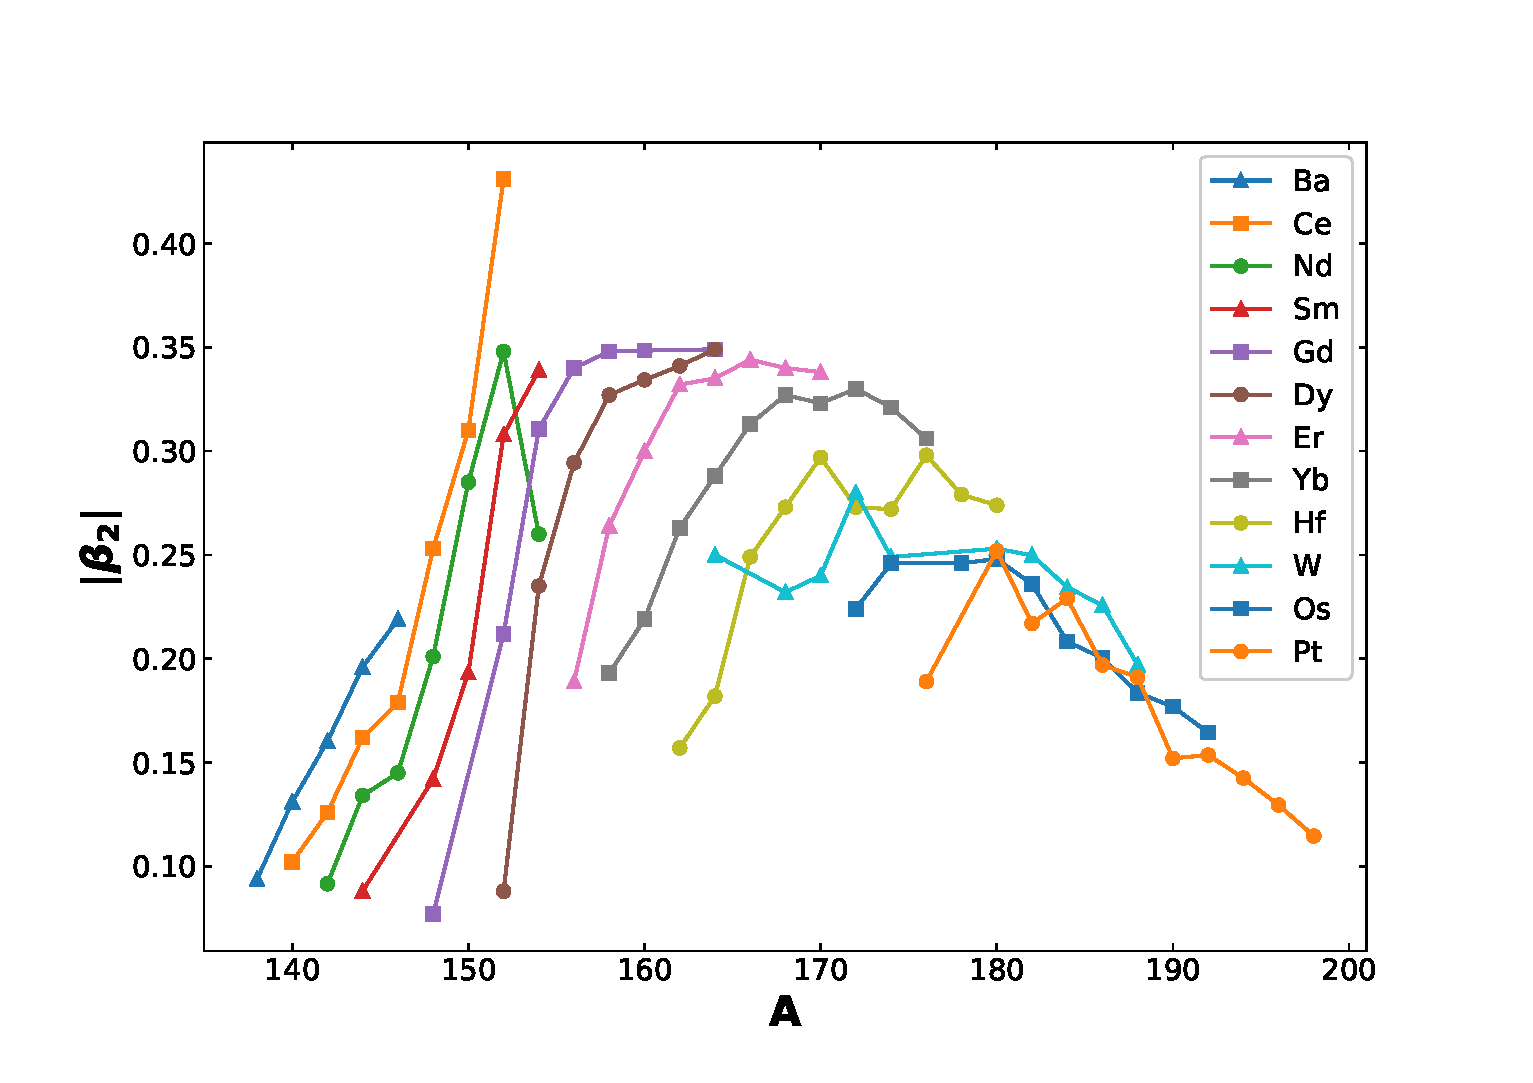
\includegraphics[scale=0.5]{Introduction_Figs/beta.eps}
    \caption{Plot of the norm of the deformation parameter $\beta_2$ along isotopic chains. Deformation can be seen setting in, as isotopic chains transition from spherical to deformed. $\beta_2$ is the quadrupole deformation parameter. The norm of $\beta_2$ is used, as the method used to calculate $\beta_2$ only gives a magnitude, not a sign. A secondary method is needed to distinguish between prolate and oblate.}
    \label{fig:beta_by_isotope}
\end{figure}